\chapter{Compose dynamic symmetry handling}\label{chap:compose}
\minitoc
\section{Composition of SP and SymmSAT}
In the previous chapter, we presented an approach that reuses the
principles of the static approaches, but operates dynamically (namely, the effective symmetry breaking approach~\cite{metin2018cdclsym}):
 the symmetries are broken during the search process without any pre-generation of the \textit{sbps}. The main
advantage of this technique is to cope with the heavy (and potentially
blocking) pre-generation phase of the static-based approaches. It also gives
more flexibility for adjusting some parameters on the fly. 
Nevertheless, we also observed that many formulas easily solved by the pure
dynamic approaches remained unsolvable by our approach and vice versa. This is
particularly true when comparing  with the \textit{symmetry propagation} technique developed by
Devriendt et al.~\cite{Devriendt12}.
Hence, our goal is to explore the composition of our algorithm with the  \textit{symmetry propagation} technique in
a new approach that would mix the advantages of the two classes of techniques while alleviating their drawbacks. At first sight,
the two approaches appear to be orthogonal, and hence could be mixed easily. However, as we show in the rest of this chapter,
this is not completely true: both theoretical and practical issues have to be analyzed and solved to get a
running complementarity. 
Since the approach based on symmetry propagation (later called SPA) focuses on
accelerating the tree traversal and the approach based on effective symmetry
breaking (later called ESBA) targets to prune the tree traversal, the question of combining these approaches, to solve a formula $\varphi$, can
be reformulated as: 
\begin{center}
 \textit{is it possible to accelerate the traversal while pruning the tree?}
\end{center}
\subsection{Theoretical foundations}
\label{sec:tf}
To answer the previous questions, we analyze the evolution of $\varphi$ during
its solving. In ESBA, $\varphi$ evolves, incrementally, to an
equi-satisfiable formula of the form $\varphi \equiv \varphi \cup \varphi_e
\cup \varphi_d$, where $\varphi_e$ is a set of injected esbps and $\varphi_d$
is a set of deduced clauses (logical consequences). Both sets are modified continuously during the solving. Hence, to be able to compose ESBA with SPA, we have to consider the symmetries of $\varphi^\prime=\varphi \cup \varphi_e \cup \varphi_d$ as
allowed permutations in place of those of $\varphi$.
A first naive solution could be to recompute, dynamically, the set of symmetries of $\varphi
\cup \varphi_e \cup \varphi_d$ for each new $\varphi_e \cup \varphi_d$, but
this would be an intractable solution generating a huge complexity. 

A  computationally less expensive solution would be to keep track of all globally unbroken symmetries as the clauses of $\varphi_e$ are injected during the solving process: considering formula $\varphi$ and 
a set of esbps $\varphi_e$ then the set of global unbroken symmetries is:
$$GUS = \underset{\omega_e \in \varphi_e}{\bigcap}Stab(\omega_e) \cap G_{\varphi}$$
 Where  $Stab(\omega_e)=\{g \in \Group \mid
\omega_e=g.\omega_e\}$ is the stabilizer set of $\omega_e$ and $G_{\varphi}$ is the set of symmetries of $\varphi$. 
Since $\varphi \cup \varphi_e  \models \varphi_d$, then $GUS$ is a valid set of symmetries for $\varphi \cup \varphi_e \cup \varphi_d$.
Then, (1) each time a new set of esbp clauses is added, its stabilizer will be used to reduce $GUS$;\label{prop:one}
(2) conversely, when a set of esbp clauses is reduced\footnote{In classical CDCL algorithm, this can be due to a back-jump or a restart.},
$GUS$ cannot be enlarged by the recovered broken symmetries because of the retrieved set:
\textit{at that point, we do not know which symmetries become valid}! 
As a consequence, the set of globally unbroken symmetries will converge very quickly to the empty set. 
At this point, SPA will be blocked for the rest of the solving process without any chance to recover.
 Therefore, this solution is of limited interest in practice.
We propose here to improve the aforementioned solution by alleviating the issue cited in point (2).
We first present the intuition, then we will detail and formalize it. 
%The idea here is to keep track of particular symmetries for each clause. For a deduced clause, this set of symmetries captures which esbp's were involved in a deduced clause's derivation. The intersection of these sets is a superset of the globally unbroken symmetries, and a strict superset after clause deletion.
Consider formula $\varphi^\prime$ as before. It can be rewritten as:
$$\varphi^\prime=\varphi \, \underset{i}{\bigcup}(\varphi_e^i \cup \varphi_d^i) \text{ , such that } \varphi_e \cup \varphi_d = \underset{i}{\bigcup}(\varphi_e^i \cup \varphi_d^i) \text{ and } \varphi \cup \varphi_e^i \models \varphi_d^i  \text{ for all } i$$
So, $GUS_i = \underset{\omega_e \in \varphi_e^i}{\bigcap}Stab(\omega_e) \cap G_{\varphi}$ is a valid set of symmetries for the sub-formula $\varphi \cup \varphi_e^i \cup \varphi_d^i$, and $GUS$ can be obtained by $GUS = \underset{i}{\bigcap} GUS_i$. If some esbp clauses are added to $\varphi^\prime$, then the new $GUS$ is computed as described in (1). The novelty here comes with the retrieval of some set of clauses: by keeping track of the symmetries associated to each sub-formula ($GUS_i$), it is now easy to recompute a valid set of symmetries for $\varphi^\prime$ when some set
$\varphi_e^k \cup \varphi_d^k$ is retrieved. It suffices to operate the intersection on the valid symmetries of the rest of the sub-formulas: $GUS = \underset{i \neq k}{\bigcap} GUS_i$.

%Just say your approach keeps track of a set of particular symmetries for each clause. For a deduced clause, this set of symmetry captures which esbp's were involved in a deduced clause's derivation. The intersection of these sets is a superset of the globally unbroken symmetries, and a strict superset after clause deletion.

\subsection{Local Symmetries}
The general and formal framework that embodies the above idea is given by the following. It first relies on the notion of \textit{local symmetries} that we introduce in \cref{def:ls}.
\begin{definition}
 \label{def:ls}
 Let $\varphi$ be a formula. We define $L_{\omega,\varphi}$, 
 the set of \textit{local symmetries} for a clause $\omega$, and with respect to 
 a formula $\varphi$, as follows:
 
 $$L_{\omega,\varphi}=\{g \in \Group \mid \varphi \models g.\omega\}$$
\end{definition}
$L_{\omega,\varphi}$ is local since the set of permutations applies locally to
$\omega$. It is then straightforward to deduce the next proposition that gives us a
practical framework to compute, incrementally, a set of symmetries for a
formula (by using the intersection of all local symmetries).
\begin{proposition}
 \label{prop:gls-prop}
 Let $\varphi$ be a formula. Then,  $\underset{\omega \in \varphi}{\bigcap}L_{\omega,\varphi} 
 \subseteq G_{\varphi}$.
\end{proposition}
\begin{proof}
 Let $\varphi$ be a formula. Then, $\forall \omega \in \varphi, \forall g \in L_{\omega,\varphi}, \varphi \models g.\varphi $. So, $\forall g \in \underset{\omega \in \varphi}{\bigcap}L_{\omega,\varphi}, \varphi \models g.\varphi$. This is combined with the fact that the number of satisfying assignments for a formula is not changed by permuting the variables of the formula, we have $g.\varphi \models \varphi$. Hence $\varphi \equiv g.\varphi$, and $g \in G_{\varphi}$ (by definition). 
\end{proof}
Using this proposition, it becomes easy to reconsider the symmetries
on-the-fly: each time a new clause $\omega$ is added to the formula $\varphi$,
we can just operate an intersection between $L_{\omega,\varphi}$ and
$\underset{\omega^\prime \in \varphi}{\bigcap}L_{\omega^\prime,\varphi}$ to get
a new set of valid symmetries for $\varphi \cup \{\omega\}$.
\medskip
Proposition \ref{prop:lsc-prop} establishes the relationship between the local symmetries of a deduced clause and those of the set of clauses that allow its derivation. 
\begin{proposition}
 \label{prop:lsc-prop}
 Let $\varphi_1$ and $\varphi_2$ be two formulas, with $\varphi_2 \subseteq \varphi_1$. 
 Let $\omega$ be a clause such that $\varphi_2 \models \omega$. Then, 
 $(\underset{\omega^\prime \in \varphi_2}{\bigcap}L_{\omega^\prime,\varphi_1})
 \cup Stab(\omega) \subseteq L_{\omega,\varphi_1}$;
\end{proposition} 
\begin{proof}
 Let us consider a clause $\omega$ and a permutation $g \in 
 (\underset{\omega^\prime \in \varphi_2}{\bigcap}L_{\omega^\prime,\varphi_1})
 \cup Stab(\omega)$.
 Since, $\varphi_2 \models \omega$, then  $g.\varphi_2 \models g.\omega$. Since $\varphi_1 \models \varphi_2 (\varphi_2 \subseteq \varphi_1)$, and 
 $g \in 
 (\underset{\omega^\prime \in \varphi_2}{\bigcap}L_{\omega^\prime,\varphi_1})
 \cup Stab(\omega)$, then we have $\varphi_1 \models g.\varphi_2$ (from Def.~\ref{def:ls}). Hence, $\varphi_1 \models g.\varphi_2 \models g.\omega$, and then, $g \in L_{\omega,\varphi_1}$ (by definition). 
\end{proof}
\subsection{Algorithm}
This section shows how to integrate the propositions developed in the previous
section as the basis of our combo approach in a concrete
Conflict-Driven Clause Learning (CDCL)-like solver.
First recall the algorithm of symmetry propagation used for the combination of two approaches.
	\begin{algorithm}[!htbp]
		
			\small	
		\SetKwProg{Fn}{function}{}{}
		\SetKwData{C}{symController}
		\SetKwData{CSP}{spController}
		\SetKwFunction{CDCL}{CDCLSymSp}
		\SetKwFunction{unitPropagation}{unitPropagation}
		\SetKwFunction{symPropagation}{symPropagation}
		\SetKwFunction{updateSymmetries}{updateActiveSymmetries}
		\SetKwFunction{cancelSymmetries}{cancelActiveSymmetries}
		\SetKwFunction{analyzeConflict}{analyzeConflict}
		\SetKwFunction{isSymmetryConflict}{isSymmetryConflict}
		\SetKwFunction{assignNewLiteral}{assignDecisionLiteral}
		\SetKwFunction{backjumpPolicy}{backjumpAndRestartPolicies}
		
	
	\Fn{
		\CDCL{$\varphi$: CNF formula, \colorsp{\CSP : symmetry propagation controller}}\\
		$\quad\quad$\textbf{returns} $\true$ if $\varphi$ is \sat and $\false$ otherwise
	}
	{
		$dl \gets 0$ \tcp*{Current decision level}
		$\alpha \gets \emptyset$\;
		\While{not all variables are assigned}{
			$isConflict \gets$ \unitPropagation{}  \
			\colorsp{$\wedge$ \CSP.\symPropagation{}}\;	\label{algo:cdclsp:symprop}
			\If{$isConflict$}{
				\If{dl = 0}{
					\Return \false
					\tcp*{$\varphi$ is $\unsat$}
				}
				$\omega \gets$ \analyzeConflict{}\;
				$dl \gets$ \backjumpPolicy{}\;
				$\varphi \gets \varphi \cup \{\omega$\} \;
				\colorsp{\CSP.\cancelSymmetries{}}\; \label{algo:cdclsp:cancel}	
			}
			\Else{
				$\alpha \gets \alpha\, \cup $ \assignNewLiteral{}\; 
				$dl \gets dl+1$\;
				\colorsp{\CSP.\updateSymmetries{}}\; \label{algo:cdclsp:update}
			}
		}
		\Return \true
		\tcp*{$\varphi$ is $\sat$}
	}
	\caption{The {\cdclsp} algorithm. Blue (or grey) parts denote additions to {\cdcl}.}
	\label{algo:cdclsp}
	
\end{algorithm}


{\cdclsp} (see Algorithm~\ref{algo:cdclsp}) implements SPA, and also has a
structure similar to the one of {\cdcl}. In this algorithm, the symmetry
propagation actions are executed by the controller component (\texttt{spController})
through a call to the function \texttt{symPropagation} (\cref{algo:cdclsp:symprop}). This
propagation is allowed only if the conditions %of Proposition \ref{prop:ws-prop}
are met. Such conditions are evaluated by tracking on-the-fly the status of the
symmetries. This is implemented by functions \texttt{updateSymmetries} (\cref{algo:cdclsp:update})
and \texttt{cancelSymmetries} (\cref{algo:cdclsp:cancel}).

\begin{algorithm}[!htbp]	
	\small	
	\SetKwProg{Fn}{function}{}{}
	\SetKwData{C}{symController}
	\SetKwData{CSP}{spController}
	\SetKwFunction{CDCL}{CDCLSymSp}
	\SetKwFunction{unitPropagation}{unitPropagation}

	\SetKwFunction{symPropagation}{symPropagation}
	
	\SetKwFunction{updateSymmetries}{updateActiveSymmetriesSym}
	
	\SetKwFunction{cancelSymmetriesSym}{cancelActiveSymmetriesSym}
	
	\SetKwFunction{updateLocSymmetries}{updateLocalSymmetries}
	
	\SetKwFunction{analyzeConflict}{analyzeConflictSymSp}

	
	\SetKwFunction{isSymmetryConflict}{isSymmetryConflict}
	\SetKwFunction{assignNewLiteral}{assignDecisionLiteral}

	\SetKwFunction{backjumpPolicy}{backjumpAndRestartPolicies}

	\SetKwFunction{isNotMinimal}{isNotLexLeader}
	\SetKwFunction{SBP}{generateEsbpSp}
	\SetKwFunction{notifyAssigned}{updateAssign}
	\SetKwFunction{notifyCancelled}{updateCancel}


	
	\Fn{
		\CDCL{$\varphi$: CNF formula, \colorsym{\C: symmetry controller},\\
			 \hspace{11em} \colorsp{\CSP : symmetry propagation controller}}\\
		$\quad\quad$\textbf{returns} $\true$ if $\varphi$ is $\sat$ and $\false$ otherwise
	}
	{

		$dl \gets 0$ \tcp*{Current decision level}
		$\alpha \gets \emptyset$\;
		\While{not all variables are assigned}{
			
			$isConflict \gets$ \unitPropagation{}  \colorsp{$\land$ \CSP.\symPropagation{}}\;\label{algo:sym_prop}
			\colorsym{\C.\notifyAssigned{$\alpha$}\;}
			\colorsym{$isReduced \gets$ \C.\isNotMinimal{$\alpha$}\;}
			
			\If{$isConflict$ \colorsym{$\vee\, isReduced$}}{
				\If{dl = 0}{
					\Return \false
					\tcp*{$\varphi$ is $\unsat$}
				}
				
				\If{$isConflict$}{\label{algo:start_stab}
					
					\colorbox{gray!30}{$\langle\omega, L = \underset{\omega' \in \varphi_1}{\bigcap}L_{\omega',\varphi_1} \cup Stab(\omega)\rangle \gets$ \analyzeConflict{}\;}
				}
				\Else {
					\colorbox{gray!30}{$\langle\omega, L = Stab(\omega)\rangle \gets$ \C.\SBP{$\alpha$}\;}
				}\label{algo:end_stab}		
				
				
				$(dl,\alpha) \gets$ \backjumpPolicy{}\;
				$\varphi \gets \varphi \cup \{\omega$\} \;
				
				\colorsym{\C.\notifyCancelled{$\alpha$}}\;
				\colorbox{gray!30}{\CSP.\cancelSymmetriesSym{}}\;\label{algo:symsp:cancel}
				\colorbox{gray!30}{\CSP.\updateLocSymmetries{L}\;}\label{algo:symsp:updateloc}
				
			}
			\Else{
				$\alpha \gets \alpha\, \cup $ \assignNewLiteral{}\; 
				$dl \gets dl+1$\;
				\colorbox{gray!30}{\CSP.\updateSymmetries{}}\;\label{algo:symsp:updateact}
			}
		}
		\Return \true
		\tcp*{$\varphi$ is $\sat$}
	}
	\caption{The {\cdclsymsp} algorithm. Additions derived
		from {\cdclsym} and {\cdclsp} are reported in red and blue (or grey). Additions
		due to the composition of the two algorithms are reported with a gray
		background.}
	\label{algo:cdclSYMSP}
\end{algorithm}
 
The algorithm we propose for the composed approach is presented in
algorithm~\ref{algo:cdclSYMSP}. 
%Lines $3$-$10$, $15$-$17$ and $20$-$22$ correspond to the exact union of {\cdclsym} and {\cdclsp}. 
Let us detail the critical points.
\begin{itemize}[topsep=2pt]
 \item \Cref{algo:start_stab}: when a conflict is detected, then the analyzing
 procedure is triggered. According to Proposition \ref{prop:lsc-prop}, the
 generated conflicting clause $\omega$, should be associated with the
 computation of its set of local symmetries. Thus, we update the classical
 \texttt{analyzeConflict} procedure to \texttt{analyzeConflictSymSp} that produces such
 a set: $\varphi_1$ contains all the clauses that are used to derive $\omega$\footnote{These are clauses of the \textit{conflict side} of the implication graph when applying the classical conflict analysis algorithm.}. So, at the end of the conflict analysis, we operate the intersection of a local symmetry of these clauses to get the set of local symmetries of $\omega$. We can thus complete this set with the stabilizer set (see Proposition \ref{prop:lsc-prop}).
 
 In the classical algorithm of symmSAT, when a non lex-leader assignment is detected, then the esbp generation function, \texttt{generateEsbp}, is
 called. In the new algorithm this function is replaced by a new one called
 \texttt{generateEsbpSp}. In addition to compute the esbp clause $\omega$, it
 produces the stabilizer set of $\omega$\footnote{The only allowed  local symmetries in case of an esbp.}.
% , according to point~2 of  section~\ref{sec:pc}.}.
 
 \item \Cref{algo:symsp:cancel}: \texttt{cancelActiveSymmetriesSym} extends function \texttt{cancelActiveSymmetries} of Algorithm~\ref{algo:cdclsp} with the additional reactivation of the symmetries that have been broken (deactivated) by ESBPA. Technically speaking, each time a deduced literal is unassigned, all symmetries that became inactive because of its assignment (see \texttt{updateLocalSymmetries} and \texttt{updateActiveSymmetriesSym} functions below) are \textit{reactivated}.
 
 \item \Cref{algo:symsp:updateloc}: \texttt{updateLocalSymmetries} is a new function of
 $\texttt{spController}$. It is responsible of updating the status of the manipulated
 symmetries so that only those respecting Proposition \ref{prop:gls-prop} are
 active each time the \texttt{symPropagation} function is called. Technically speaking, each symmetry of the complement set (to $G_{\varphi}$) of the set $L$ is marked \textit{inactive} (it is a broken symmetry), if it is not already marked so. Here, the asserting literal of clause $\omega$ becomes responsible of this deactivation. 
 
 \item \Cref{algo:symsp:updateact}: \texttt{updateActiveSymmetriesSym} extends function \texttt{updateActiveSymmetries} of algorithm~\ref{algo:cdclsp}. The reason clause, $\omega_l$, of each propagated literal, $l$, by the \texttt{unitPropagation} function is analyzed. Each symmetry of the complement set (to $G_{\varphi}$) of the set local symmetries of $\omega_r$ is marked \textit{inactive}, if it is not already marked so. $l$ becomes responsible of this deactivation. 
\end{itemize}


\subsection{Illustrative Example}

Consider the following permutation $G = \{ g_1 = (x_1 x_2) (x_3 x_4)  , g_2 = (x_3 x_4) (x_5 x_6) \}$,
the lexicographic ordering relation of variables with $\true < \false$ and 
the current assignment $\alpha = \{\neg x_7 \}$.
Suppose the permutation $g_1$ already generate the $esbp$ $\omega_e = \{ x_1 \neg x_2\}$ then, associated local symmetry is 
$g_2$ because it stabilizes $\omega_e$ ($g_2.\omega_e = \omega_e)$. Then, suppose a conflict occurs and the resulting clause is
$\omega_d = \{x_4\, x_7\}$. In the conflict analysis, this clause is deduced by original clauses and $\omega_e$.
 So, it have the same valid symmetries as $\omega_e$. As $g_2.\omega_d = \{x_3\, x_7\}$ is an assertive clause and $g_2$ is a valid 
 permutation for this clause SP can propagate $x_3$ (the symmetrical of $\omega_d)$



\subsection{Implementation}
We have implemented our combo on top of the
\texttt{minisat-SPFS}\footnote{https://github.com/JoD/minisat-SPFS} solver,
developed by the authors of SPA.
This choice has been influenced by two points: (1) take advantage of the
expertise used to implement the original SPA method; (2) the easiness of
integrating our implementation of ESBA to any CDCL-like solver (because it is an
off-the-shelf library\footnote{This library is released under GPL v3 license,
see \url{https://github.com/lip6/cosy}.}).
However, this choice has the drawback of doubling the representation of
symmetries. This can be a hard limit to treat certain big problems from the
memory point of view.
The implemented combo solver can be found at:\\
\mbox{\url{https://github.com/lip6/minisat-SymSp}}
\subsection{Evaluation}
This section compares our combo approach against ESBA and SPA. All experiments
have been performed with a modified version of the well-known \minisat{} solver \cite{een2003extensible}: \texttt{minisat-Sp}, for
SPA; \texttt{minisat-Sym}, for ESBA; and \texttt{minisat-SymSP}, for the
combo. Symmetries of the SAT problems have been computed by
\bliss{}~\cite{JunttilaKaski:ALENEX2007}.

We selected from the last seven editions of the SAT contest
\cite{jarvisalo2012international}, the CNF problems for which \bliss{} finds
some symmetries that could be computed in at most $1000s$ of CPU time. We
obtained a total of $1400$ SAT problems (discarding repetitions) out of the
$4000$ proposed by the seven editions of the contest (from 2012 to 2018).
\begin{table}\footnotesize
 \centering
 % \resizebox{1 \textwidth}{!}{
 \begin{tabular}{l|ccc}
  \toprule
  Benchmark  &\texttt{minisat-Sp} & \texttt{minisat-Sym} & \texttt{minisat-SymSP}\\
  \hline 
  Generators 0–20 (704) & 194&197&\cellcolor{gray!30,}\textbf{198}\\
  Generators 20–40 (136) & 33&\cellcolor{gray!30}\textbf{34}&\cellcolor{gray!30}\textbf{34}\\
  Generators 40–60 (141) & 28&28&\cellcolor{gray!30}\textbf{29}\\
  Generators 60–80 (168) & \cellcolor{gray!30}\textbf{65}&64&\cellcolor{gray!30}\textbf{65}\\
  Generators 80–100 (51) & 28&\cellcolor{gray!30}\textbf{34}&\cellcolor{gray!30}\textbf{34}\\
  Generators  \textgreater100 (200) & 58&59&\cellcolor{gray!30}\textbf{60}\\
  \hline 
  TOTAL no dup (1400) & 406 & 416 & \cellcolor{gray!30,}\textbf{420}\\
  \bottomrule
 \end{tabular}
 % }
 \caption{Comparison of the number of SAT problems solved by each approach.}
 \label{tab:sat}
\end{table}
\begin{table}\footnotesize
 \centering
 % \resizebox{1 \textwidth}{!}{
 \begin{tabular}{l|ccc}
  \toprule
  Benchmark  &\texttt{minisat-Sp} & \texttt{minisat-Sym} & \texttt{minisat-SymSP}\\
  \hline 
  Generators 0–20 (704) & \cellcolor{gray!30,}\textbf{233}&220&226\\
  Generators 20–40 (136) & 50&\cellcolor{gray!30}\textbf{54}&\cellcolor{gray!30}\textbf{54}\\
  Generators 40–60 (141) & 75&\cellcolor{gray!30}\textbf{83}&\cellcolor{gray!30}\textbf{83}\\
  Generators 60–80 (168) & \cellcolor{gray!30}\textbf{11}&\cellcolor{gray!30}\textbf{11}&10\\
  Generators 80–100 (51) & \cellcolor{gray!30}\textbf{11}&\cellcolor{gray!30}\textbf{11}&\cellcolor{gray!30}\textbf{11}\\
  Generators \textgreater100 (200) & 90&\cellcolor{gray!30,}\textbf{109}&107\\
  \hline 
  TOTAL no dup (1400) & 470&488&\cellcolor{gray!30,}\textbf{491}\\
  \bottomrule
 \end{tabular}
 % }
 \caption{Comparison of the number of UNSAT problems solved by each approach.}
 \label{tab:unsat}
\end{table}

All experiments have been conducted using the following settings: each solver
has been run once on each problem, with a time-out of 7200 seconds (including
the execution time of symmetry generation) and limited to 64 GB of memory.
Experiments were executed on a computer with an Intel Xeon Gold 6148 CPU
@ 2.40 GHz featuring 80 cores and 1500 GB of memory, running a Linux 4.17.18,
along with g++ compiler version 8.2.

Tables \ref{tab:sat} and \ref{tab:unsat} present the obtained results for SAT
and UNSAT problems respectively. The first column of each table lists the
classes of problems on which we operated our experiments: we classify the
problems according to the number of symmetries they admit. A line noted
``generators X-Y (Z)'' groups the Z problems having between X and Y generators
(i.e., symmetries). Other columns show the number of solved problems for each
approach.
Globally, we observe that the combo approach can be effective in many classes
of symmetrical problems. For SAT problems, the combo has better results than the
two other approaches (4 more SAT problems when compared to the best of the two
others) and this is despite the significant cost paid for the tracking of the
symmetries' status. When looking at the UNSAT problems, things are more
mitigated. Although, the total number of solver problems is greater than the
best of the two others, we believe that the cost for tracking the symmetries'
status has an impact on the performances. This can be observed on the first and
last lines of Tables~\ref{tab:unsat}: when the number of generators is small
(first line), the ESBA benefits greatly from the SPA. When the number of
generators is high (last line), we see a small loss of the combo with respect
to ESBA. It is also worth noting that the combo approach solved \textbf{8} problems 
that could not be handled by ESBA nor SPA.
%These observations are confirmed by the scatter plots of Fig.\textcolor{red}{X}.
\begin{table}[!htbp]
 \begin{center}
  \resizebox{0.5 \textwidth}{!}{
   \begin{tabular}{lcc}
    \hline
    Solvers                  &    PAR2 (1400) &   CTI (825) \\
    \hline
    \texttt{minisat-SymSp}   & \cellcolor{gray!30}{5,653,089} &      614,856 \\
    \texttt{minisat-Sym}             & 5,682,892 &      \cellcolor{gray!30,}{584,868} \\
    \texttt{minisat-Sp}             & 6,026,840 &      612,638 \\
    \hline
   \end{tabular}
  }
 \end{center}
 \caption{Comparison of PAR-2 and CTI times (in seconds) of the global solving.}
 \label{tab:global}
\end{table}
Table~\ref{tab:global} compares the different techniques with respect to the
PAR-2 and the CTI time measures. PAR-2 is the official ranking measure used in
the yearly SAT contests~\cite{jarvisalo2012international}. CTI measures the
Cumulative solving Time of the problem Intersection (i.e., 825 problems solved
by all solvers). While PAR-2 value gives a global indication on the
effectiveness of an approach, CTI is a good mean to evaluate its speed compared
to other approaches.
Hence, we observe that the combo has a better PAR-2 score, and this shows its
effectiveness. However, it is the least fast when coming to solved intersection.
This is clearly due to the double cost paid for tracking the symmetries' status
(one for ESBA and the other for SPA). Having a unified management of
symmetries tracking would probably reduce this cost.
\begin{center}
\begin{figure}[!htbp]
 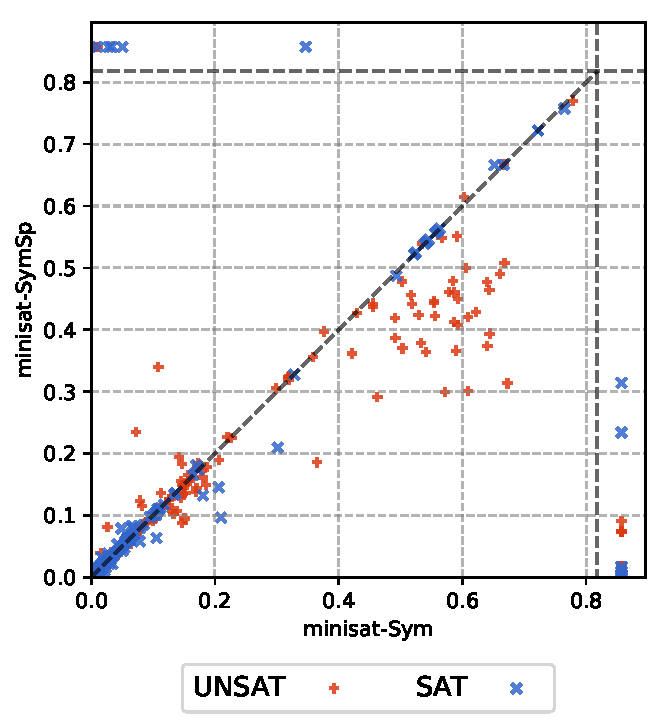
\includegraphics[scale=0.5]{img/full-INFGB-ratio-vscosy.pdf}
 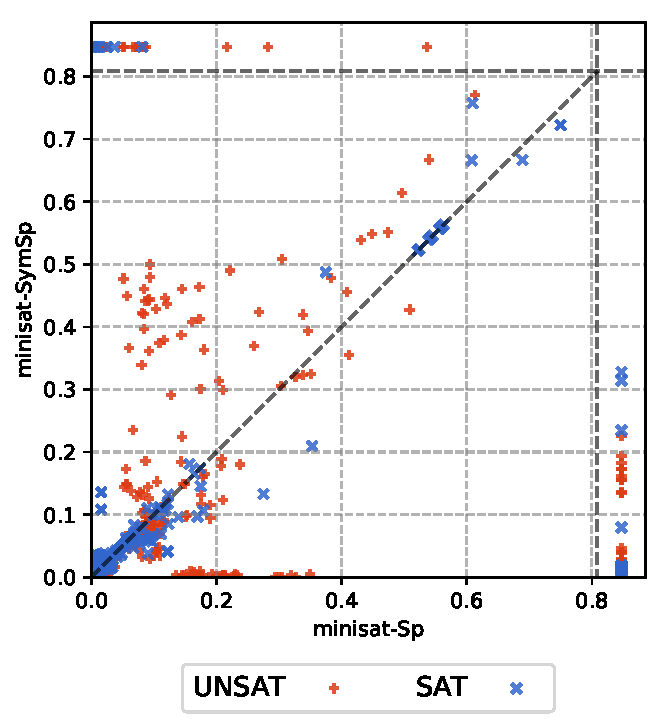
\includegraphics[scale=0.5]{img/full-INFGB-ratio-vsspfs.pdf}
 \caption{Comparison of the ratio between the number of decisions and the number of propagation for the combo w.r.t. ESBA and SPA.}
 \label{fig:ratio}
\end{figure}
\end{center}

To go further in our analyze, we also compared the ratio between the number of
decisions and the number of propagation. This is a fair measure to assess the
quality of a SAT solving approach: if the ratio is small, then this means that
the developed algorithm is producing more deduced facts than making guesses,
which is the best way to conclude quickly on a problem!
The scatter plots of Fig.\ref{fig:ratio} show a comparison between the
aforementioned ratios. When comparing \texttt{minisat-Sp} to
\texttt{minisat-SymSp} (right hand side scatter plot), we observe that the
ratio goes in favor of \texttt{minisat-Sp} for the problems solved by both
approaches. This is an expected result since the main objective of SPA is to
minimize the number of decisions while augmenting the number of propagation.
What is important to underline here is highlighted on the left hand side
scatter plot: on a large majority of UNSAT problems, the ratio goes in favor
of \texttt{minisat-SymSp} w.r.t. \texttt{minisat-Sym}. This confirms the
positive impact of SPA when applied in conjunction with ESBA.


\hakan{Mettre cela en future works dans la conclusion finale}

\section{Another combo approach}
Introducing local symmetries allow us to use it with another dynamic approach : 
\textit{Symmetry Explanation Learning} (SEL). It computes the symmetrical learning clause and
include it in the solver clauses when it can be used in the unit propagation or leads to a conflict.
With local symmetries, each clause has a set of allowed symmetries, when a symmetry wants to 
add a symmetrical clause, it suffices to check if this permutation belongs to local symmetries.

 
\section{Exploitation of local symmetries}
Local symmetries seen previously allows to exploit symmetries in different ways.
Effectively, we can consider symmetries on a part of the problem. Only clauses that are really used
by the solver i.e in the implication graph can be processed.
To obtain the symmetries of the current sub problem is the intersection of local symmetries.